% Created 2019-03-02 sáb 10:07
\documentclass[11pt]{report}
\usepackage[utf8]{inputenc}
\usepackage[T1]{fontenc}
\usepackage{fixltx2e}
\usepackage{graphicx}
\usepackage[catalan]{babel}
\usepackage{longtable}
\usepackage{float}
\usepackage{wrapfig}
\usepackage{rotating}
\usepackage[normalem]{ulem}
\usepackage{amsmath}
\usepackage{textcomp}
\usepackage{marvosym}
\usepackage{wasysym}
\usepackage{amssymb}
\usepackage{hyperref}
\graphicspath{{./images/}}

% This package is used for pretty printing the source files. 
% Edit to taste.
\usepackage{listings}
\usepackage{color}
\definecolor{mygreen}{rgb}{0,0.6,0}
\definecolor{mygray}{rgb}{0.5,0.5,0.5}
\definecolor{mymauve}{rgb}{0.58, 0, 0.82}
\lstset {
  numbers = left,
  numberstyle = \tiny\color{mygray}, 
  emphstyle = \bfseries,
  commentstyle=\color{mygreen},
  keywordstyle=\color{blue},
  language=Octave,
  rulecolor=\color{black}, %if not set the frame-color may be changed on line-breaks within not-black text
  title=\lstname,
  stringstyle=\color{mymauve}
}
\tolerance=1000
\author{David Márquez\and Irene Mollet the best}
\date{\today}
\title{Pràctica 1\\Pseudorandom Noise Generator}
\newcounter{previCounter}
\newenvironment{enunciat}{
  \stepcounter{previCounter}
  \par\vspace{\baselineskip}\noindent
  {\bf Tasca~\thepreviCounter.}}{\par\medskip\ignorespacesafterend}
\begin{document}

\maketitle

\section*{Using the sound card from Octave}
\begin{enunciat}
What is the length of the played sound if you use a sampling frequency Fm different that the
one you have used to record the sound?
\end{enunciat}

\section*{Noise with normally distributed values}
\begin{enunciat}
Play with randn.m to know what a normally distribution is.
\end{enunciat}
Sona com el soroll?


\section*{Noise with binary values}
\begin{enunciat}
Comparar si x2 i x1 sonen similars (x2 és binari)
\end{enunciat}

\section*{Noise with binary values using LFSR}
Captura del codi 
Diferències entre les diferents n i a partir de quina n es comença a sentir normal.
Explicar perquè.


\section*{Spectrum of the noise}

Entre quines Fm em variat i quines son les diferències.
Captures dels espectres






\section*{Advanced activity}

Diferencies de so entre els dos senyals
Fotos oscil·loscopi.
Explicació fotos



%MEMORIA OKEY A PARTIR D'AQUI------------------------------------------------------------------------------------------------------------
\section*{Introducció}
En aquesta pràctica s'estudiaran diferents aspectes de les seqüències pseudoaleatories de soroll.



\section*{Assaig arxiu1.m}
\begin{enunciat}
     Visualitzeu i escolteu el senyal generat per a diferents freqüències de mostreig i per a diferents valors de n.
\end{enunciat}
Els senyals x1, x2 i x3 són tres senyals basats en seqüències pseudoaleatòries generades de diferents maneres.
x1 s'ha generat a partir de la funció \texttt{randn}, la qual retorna una matriu de \texttt{Nx1} valors pseudoaleatoris.
x2 és un vector basat en el vector x1, però convertint tots els seus valors en v0 o v1. En aquest cas v0 = -1 i v1 = 1, ja que d'aquesta manera s'aprofita tot el rang dinàmic de la tarja de so de l'ordinador.
x3 també és un vector binari de longitud ${2^n-1}$, generat a partir d'un liner feedback shift register (LFSR a partir d'ara).
\paragraph{}
Per poder generar aquests senyals d'una manera fàcil s'ha creat dues funcions que s'utilitzen en els fitxers \texttt{arxiu1.m} i \texttt{arxiu2.m}.
La funció per generar x1 i x2 és senzilla, ja que només ha d'utilitzar la funció randn per generar la seqüència pseudoaleatòria.
La funció per calcular x3 és més complicada, perquè ha d'implementar el LFSR. Per fer-ho s'ha creat una funció que únicament crea la seqüència numèrica.

\lstinputlisting {LFSRs.m}
Com es pot veure, es pot utilitzar per diversos valors de n. D'aquesta manera s'ha pogut comprovar què passava quan canviaven els valors de n.
\paragraph{}
El programa que s'encarrega de calcular x3 calcula el nombre de mostres necessàries de la següent manera:
\begin{equation}
     N = (2^{n} - 1) * ceil\Big(\frac{tf * Fm}{2^{n} - 1}\Big)
\end{equation}

D'aquesta manera es pot veure correctament el senyal en l'espectre freqüencial. El que fa és que el nombre de mostres sempre sigui un múltiple del del període en bits ($2^n - 1$) de la seqüència generada amb el LFSR.

El valor de n equival al nombre de registres del LFSR. Per cada nombre de registres hi ha un polinomi que determina com s'han de col·locar les XOR per obtenir el màxim període de bits. Per tant el valor de n ens diu la freqüència amb la qual es repetirà el soroll. Per aquesta raó està directament relacionat amb la freqüència de mostreig. Com més gran és la freqüència de mostreig més ràpid es repetirà el patró. Per exemple, si utilitzem n=16 (període equival a 65535 bits), i una freqüència de mostreig de 96KHz, veiem que podrem escoltar el patró repetit $\frac{96000}{65535}=1.46$ vegades cada segon. És a dir que si mostrem el senyal durant dos segons, es podrà escoltar el patró repetit 3 vegades aproximadament.
\paragraph{}
Podem extreure, doncs, que $Fo=\frac{Fm}{2^n-1}$. L'espectre és un tren de deltes (idealment es mostreja amb deltes) situades a la freqüència fonamental i als seus harmònics (Fo, 2Fo, 3Fo, etc.). Per tant quan n augmenta, si $Fm$ es manté constant, Fo s'aproxima a 1Hz. A 1Hz, la oida humana ja no nota gairebé la diferència (la resolució de l'oïda humana és d'aproximadament 3.6KHz), i per tant per a nosaltres, l'espectre freqüencial sembla constant, igual que el del soroll blanc. Per aquesta raó com més alta és la n més s'assembla al soroll blanc.
\paragraph{}
Hem comprovat que a partir de n = 13, no escoltem la diferència. Amb n = 13 i una freqüència de mostreig de 48KHz veiem que Fo ens dóna 5.86Hz, un valor molt proper a la resolució màxima de l'oïda humana.

\paragraph{}
Per altra banda, s'ha canviat Fm deixant n constant. El resultat ha estat que amb Fm molt baixes (12 i 24 KHz) el so se sentia sense aguts.
Això és degut al fet que per mostrejar un senyal correctament es necessita una freqüència mínima de $2Fa$. Si mostrejam a 12KHz només es podrà sentir el senyal fins a 6KHz (vegeu \ref{fig:Fm12}).
\begin{figure}[h]
\label{Fm12}
  \centering
  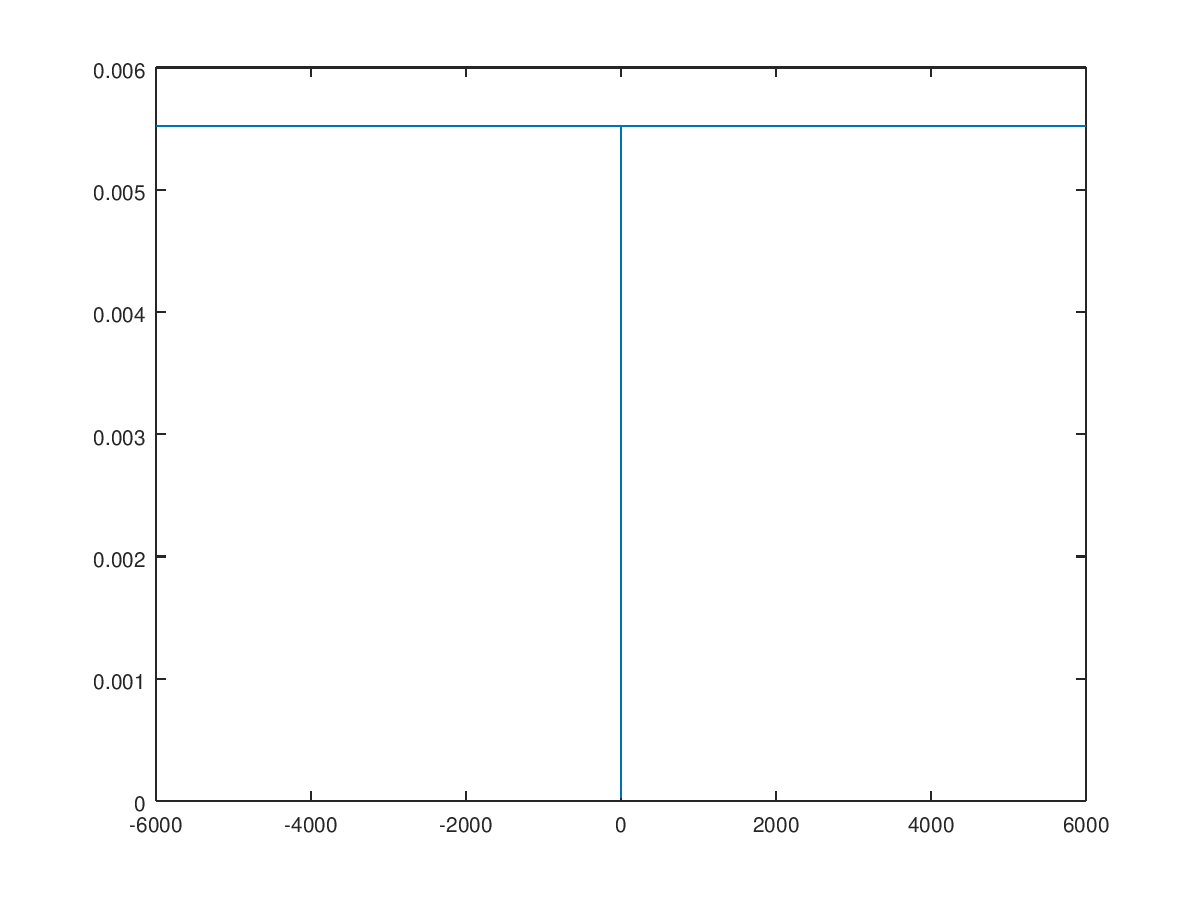
\includegraphics[width=0.5\textwidth]{img/Fm12}
  \caption{LFSR, n=16, Fm=12KHz}
\end{figure}

\section*{Assaig arxiu2.m}


En el cas on x3 és una seqüència de [-1 1 1] repetida N vegades, en el seu espectre es pot veure una delta a cada Fo.
Per x4, que és la mateixa seqüència amb cada element repetit nr vegades,passa el mateix (Fo és la mateixa), però per les freüències múltiples de Fm4, la delta és nul·la.




NOSE EL PERQUÈ

Quan x3 és un senyal pseudoaleatori generat pel SLRF, x4 



Compareu x3 amb x4 (espectre i audio) per a diferents valors dels paràmetres Fm, n i nr.


A les següents captures de l'oscil·loscopi es pot veure com el senyal x4 és més "polit" que el x3. Això es degut a que el x4 té mes resolució.

A l'espectre del senyal x4 es pot observar com és 0 quan F és Fm3
\section{Conclusions}



\end{document}
%\begin{figure}[h]
%  \centering
%  \includegraphics[width=0.5\textwidth]{x2-amp2}
%  \caption{Senyal de veu original ampificat }
%\end{figure}
